\documentclass[12pt,oneside,a4paper]{article}
%
\usepackage{graphicx}
\usepackage{tabularx}
\usepackage{url}
\usepackage[latin1]{inputenc}
%\usepackage[utf8]{inputenc}
\usepackage[left]{eurosym} 
\usepackage{times}
\usepackage{pdfpages}
\usepackage{todonotes}
\usepackage{enumerate}

% We don't want a special font for urls (looks bad with times):
\urlstyle{same}

% Graphics extensions and path:
%\DeclareGraphicsExtensions{.pdf,.png,.jpg}
%\DeclareGraphicsExtensions{.eps,.ps}
%\graphicspath{{figures/}}

%
% Page size
%
\usepackage[top=25mm,left=25mm,right=25mm,bottom=25mm]{geometry}

\setlength{\headheight}{15pt}    % Necessary to avoid fancyhdr warning.


\newcommand\LongTitle{Humidity, clouds and snow in the Arctic}
\newcommand\ShortTitle{Humidity, clouds and snow in the Arctic}



%
% Heading
%
\newcommand{\pagevers}[2]{
\ifnum\thepage=1 
#1
\else#2
\fi
}
%
\usepackage{fancyhdr}
\pagestyle{fancy}
\chead{}
%\rhead{\pagevers{}{\bf \thepage}}
\rhead{\thepage}
\rfoot{\small \it \ShortTitle\ ---\  Application to SNSA 2021-R}
\cfoot{}
\lfoot{}
%\renewcommand{\headrulewidth}{\pagevers{0pt}{0.2pt}}
\renewcommand{\headrulewidth}{0.2pt}
\renewcommand{\footrulewidth}{0pt}


\newcommand{\docname}[1]{\lhead{\small #1}}

%
% Section titles
%
\usepackage[small]{titlesec}
\titlespacing*{\section}{0pt}{*3.3}{*0.5}
%
% 
%
\def\compactitems{\parskip0pt\topsep0pt\partopsep0pt\parsep0pt\itemsep0pt}

% Struts for better table formatting:
\newcommand\T{\rule{0pt}{2.6ex}}
\newcommand\B{\rule[-1.2ex]{0pt}{0pt}}


\newcommand{\FIXME}[1]{{\bfseries \textcolor{red}{FIXME:} #1}}
\newcommand{\md}[1]{\mbox{#1-d}}
%\newcommand{\3d}{3d}

%\hyphenation{3-d}
\uchyph=0

%%% Local Variables: 
%%% mode: latex
%%% TeX-master: t
%%% End: 



\docname{Project description}
\usepackage{graphicx}
\usepackage{caption}
\usepackage{subcaption}
\usepackage{multirow}
\usepackage{amsmath}
\usepackage{booktabs}
\captionsetup[figure]{font=small,labelfont=small}

%
% References
%
\usepackage{natbib}
\bibliographystyle{agu04}     
\setlength{\bibsep}{0mm}


\newcommand\wpstart[3]{\noindent\textbf{WP #1, #2}\hspace{\stretch{1}}Priority #3%
	\vspace{-4mm}\\\rule{\textwidth}{0.5pt}\\}
\newcommand\wpenda[4]{%
	\noindent -----\\ 
	\begin{tabularx}{0.95\hsize}{l p{133mm}}    
		\hspace*{-1.1ex}Start\,--\,end: & #1\\
		\hspace*{-1.1ex}Main output: & #2\\
		\hspace*{-1.1ex}Main risks: & #3\\
	\end{tabularx}\\
	\vspace{-2.2ex}\noindent\rule{\textwidth}{0.5pt}\\
}


\newcommand\intodo[1]{{\color{red} [* #1 *]}}


\begin{document}
	
	
	\thispagestyle{empty}
	\vspace*{-10mm}
	\noindent
	\textbf{\Large \LongTitle}




\section{General summary}
%
The Arctic is a water world, experiencing rapid warming. Passive microwave
satellite measurements are required for a comprehensive view of the different forms of water in the region. The project targets water in the atmosphere, and the basic aim is to improve the utilisation of this data source, particularly by using high-frequency observations. The proposed retrieval system is highly versatile and retrievals of other water forms like liquid water content, snowfall, and sea-ice concentration (in order of priority) are also feasible.

We propose a physically-based, Bayesian-oriented, machine-learning model for
the task. The model is trained with detailed 3D radiative transfer simulations,
to generate local scenes of measured radiances. The input to the simulations
has a horizontal resolution finer than the size of the satellite footprints.
For example, high-resolution SAR (synthetic-aperture radar) imagery is applied
to describe the distribution of sea-ice\,/\,open water at a resolution of
200\,m. As a result, aspects like inhomogeneous surface types and overlap of
the footprints are incorporated into the simulations and are then automatically
considered in the retrieval process, in contrast to existing retrieval methods.
Precipitation and clouds are modelled in detail by combining a mesoscale model
with the in-house expertise on microwave radiative transfer involving
hydrometeors. As we cover all significant parts of the ``forward problem'', our
inversions can be truly ``all-sky''; we aim for a zero data rejection (for the
set of channels included).

The resulting dataset(s) would play an important role in not only analysing the
variability of water above the Arctic, but also in deciphering the
ongoing trends involved in the Arctic amplification of global warming.


%Water vapour plays an important role in the water and energy cycle over the polar regions, especially over Arctic. Over the Arctic, changes in the water vapour content are most sought to observe the warming trends, also know and Artic amplification. However over poles, the ground measurements are sparse and the performance of the satellite retrievals is constrained by the highly variable surface emissivity. The basic aim of this project is to develop new retrieval algorithms principally for total water vapour (TWV) from satellite microwave radiometer data over the Arctic. We propose a physically based retrievals, using a Bayesian machine learning based inversion method. Additionally, this algorithm could be used to also retrieve side products like total liquid water content (LWC) and sea-ice concentration (SIC). A key feature of this algorithm would be the use high resolution SAR imagery to classify sea-ice and open waters. Fine scale sea-ice information is necessary for distinguishing emissivity between different surface types. Another crucial aspect of the development line will be to use data from multiple microwave frequencies, with different footprint size, and avoiding the remapping of data. The overall scheme shall be similar to the one in a parallel SNSA 2021 proposal submitted by co-applicant Patrick Eriksson.
%The resulting dataset would play an important role in not only analysing the water vapour variability of the Arctic atmospheric but also in deciphering the trends the Arctic climate change.


\subsection{Background}
%
\label{sec:background}
The Arctic is a very sensitive region to climate change and has a significant
influence on the mid-latitudes, e.g.\ European weather patterns. In the recent
years an amplified warming (2-3 times higher compared to the rest of the world)
has been observed in this region (Arctic amplification), which is caused by
unique feedback processes influencing the Arctic climate. Unfortunately
detailed knowledge on the feedback processes is still missing and the scarcity
of observations in the Arctic makes it difficult to assess the situation and
processes taking place. However, water vapour and the increase in water vapour
in the last decades due to decreasing sea ice cover seems to be one of the key
players of Arctic feedback processes \citep[e.g.][]{ vihma:2016:theat}. A decrease in sea ice leads to an increased uptake of solar
radiation of the Arctic ocean which enhances the heat flux from the ocean to
the atmosphere and the amount of water vapour in the air, a greenhouse gas that
can induce further warming and melting of the sea ice \citep{screen:2010:thece}. In
addition to its role as a greenhouse gas, water vapour is also relevant when it
comes to the water cycle in the Arctic, i.e. clouds and precipitation which
have an impact on surface temperature and sea ice as well
\citep{blanchet:water:1995}. To understand and monitor water vapour in the
Arctic, its role for the Arctic water cycle and its climate impact,  observations
are needed. Conventional observations such as radiosondes have a substantial
impact on the numerical weather prediction of the Arctic
\citep{lawrence:2019:usean}, but they are not able to provide a comprehensive
spatial coverage as satellites can do.

\subsection{Previous work}
%
\label{sec:previousworks}
%
Over the Arctic, polar orbiting satellites provide the most dense coverage
of observations, both by infrared and microwave instruments. As the area
experiences polar night and has extensive cloud cover, optical and infrared
techniques suffer from basic limitations; thus to avoid these issues, only
satellite-based passive microwave data are considered in the proposed project. Over the polar regions, a challenge encountered by passive microwave observations is the high and highly variable contribution by surface emission.

The most extensive work towards stand-alone retrievals of water vapour path
(WVP) over the Arctic using microwave humidity sounders (such as Advanced
Microwave Sounding Unit-B (AMSU-B) and Microwave Humidity Sounder (MHS) comes
from University of Bremen. Their retrieval concept was initiated by
\citet{miao:2001:atmos}, where they utilized water vapour absorption channels
around 183\,GHz and the 150\,GHz window channel to retrieve WVP upto 7\,kg\,m$^{-2}$. Subsequently \citet{melsheimer:2008:impro} extended this approach to
include 89\,GHz to retrieve WVP up to 15\,kg\,m$^{-2}$ over sea-ice regions.
They used data from measurement campaigns to formulate a relationship between
sea-ice emissivity over different frequencies. Later,
\citet{scarlat:2018:retri} extended the method to include all surface types
using AMSU-B. A comparison of the retrieved WVP against ERA-Interim reanalyses
showed that the over winter months, the mean differences were 1.86\,kg m$^{-2}$
but over summer months the errors were up to 5.67\,kg m$^{-2}$, due to the
algorithm being constrained by its upper retrieval limit of 15\,kg m$^{-2}$.
Further, an attempt has also been made to use low frequency microwave
observations from the Advanced Microwave Scanning Radiometer (AMSR). For example,
\citet{scarlat:2017:exper} use optimal estimation for multi-parameter retrieval
over Arctic, and \citet{zabolotskikh:2020:anadv} attempt WVP retrievals over
both open ocean and sea-ice regions using neural networks based inversion. In
both the products, the highest uncertainties are linked to the empirical
estimates of surface emissivity over sea-ice regions. In fact, the skill of all
available satellite-based water vapour retrievals in this region is highly
variable over different atmospheric and surface conditions. For example, in the
central Arctic, for summer months, the monthly means derived from different
satellite products can differ up to 30\% \citep{crewell:2021:asyst}.

The frequent sampling of polar orbiting satellite data over the Arctic carries
huge potential at improving numerical weather prediction (NWP).
\citet{lawrence:2019:usean} show that over the summer months, assimilation of
microwave sounding observations leads to more than 3\% reduction in the total
global forecast error, but during winters, their impact reduces to 2\%, as
almost 24\% of the microwave observations are rejected. The high rejection rate
in the winter season is a consequence of the forward model errors associated
with the estimation of surface properties particularly over snow and sea-ice,
and the high forecast model errors \citep{bauer:2016:aspec}. Thus, efforts are
required to bridge the gap between the seasons. Further, despite that
reanalyses based on NWP show good skill for WVP, vertical profiles can be
systematically wrong and cloud fractions are poorly predicted, with large
impact on the surface radiative fluxes driving melting of ice
\citep{graham:2019:evalu}. Increasing the usage of satellite data over all
surfaces in the Integrated Forecast System (IFS) is also identified as one of the
priorities in ECMWF (European Centre for Medium-Range Weather Forecasts)
Strategy for 2021-2030.



\subsection{The way forward: Problems and solutions }
%\subsubsection{Problems and solutions}

Remote sensing provides indirect measurements and the data retrieval always
offers some degree of complexity. When using passive satellite microwave data
to estimate humidities over the Arctic region, the main limiting factor is the
surface's contribution to measured radiances. The special role of the surface
is due to high atmospheric transmissivities and the difficulties to predict the
surface properties of snow (on either land or ice). The main solution today is
to reject channels with a significant surface contribution. This gives a low
utilisation rate of the satellite data, and leaves the humidity close to the
surface unconstrained.

For this reason, efforts are being made to improve the ``forward modelling'',
i.e.\ use auxiliary data to predict the local radiative properties of snow and
sea-ice. This constitutes a very hard problem as the properties depend on a
high number of snow and sea-ice variables. There will be progress in this area,
but it is likely to be slow. Another less discussed aspect is that individual
satellite footprints can cover both sea ice and open water. To handle this, the
information from a large scale ice-fraction is not sufficient, even the
distribution of ice and water inside the footprint matters. This makes
retrievals above surface types like open leads and polynyas particularly
problematic. The risk of having an inhomogeneous footprint increases with
footprint size, thus a good spatial resolution is advantageous even if the
atmospheric fields show little horizontal variability.

We will attack these issues from a new angle, now feasible due to progress in
machine learning (ML). We avoid the limitations in traditional approaches by
basing the inversions on a retrieval database, which is used to train the ML
model. The simulated measurements in the database are generated on
high-resolution data, thus the variations of both surface and atmospheric variables
inside the footprint get included. In addition, by simulating "scenes" of
adjacent footprints, and not just individual ones, the information hidden in
the overlap of footprints can be exploited. The latter effectively increases the
horizontal resolution, but also provides background spatial information, such
as indications on if the surface is homogeneous or mixed.


\section{Project description}
%
\subsection{Scientific objectives and considerations}
The main objective of this study is to provide physical, stand-alone, water
retrievals over the Arctic from passive microwave instruments, which can be
comparable to or better in performance than existing reanalyses and satellite
based products. The basic idea is to combine a database based on sophisticated
3D radiative transfer with ML to retrieve water properties and estimate the
associated uncertainties. The primary aim is to estimate humidity, however, a
simultaneous retrieval of liquid water content will also be undertaken as a
second priority. Nonetheless, before going ahead, it is crucial to elucidate
the following:
\begin{itemize}
 \vspace{-1ex}
\item The region north of Arctic Circle ($66^{\circ}33^{'}$N) will be defined
  as the Arctic region.
 \vspace{-1ex}
\item The retrieval database will work like the prior assumptions in a standard
  Bayesian retrieval, but by using ML we will not be restricted to Gaussian
  statistics. ML can handle strong non-linear problems, and we can include
  aspects that are very difficult to handle in traditional retrievals (such as
  inhomogeneous footprints). It is not needed to predict the conditions exactly
  where the observation is made, it is sufficient for the simulations to have a
  similar variability as reality. The ML algorithm uses the database provided
  to give the posterior knowledge of the quantity sought, given the scene of
  observations.
 \vspace{-1ex}
\item We will invert all observations. For certain conditions some channels
  will not provide any useful information due to interference of the surface or
  e.g.\ heavy snowfall. Our retrievals will then fall back to the prior
  information embedded in the database in a stable manner and a proper
  uncertainty estimate can still be given. The key here is that the disturbing
  factors are included in the simulations. This in contrast to other retrievals
  where forward model errors not are properly described and e.g.\ including
  surface sensitive channels can easily lead to a totally unphysical retrieval.
  \vspace{-1ex}
\item If useful additional information becomes available during the course of
  the project, it can be incorporated into the ML training. For example, if
  there is progress in snow modelling and the local emissivity can be estimated
  with some certainty, this can be seen as a virtual measurement and be used to
  improve the ML model.
\end{itemize}


\subsection{Data and tools}
% 
\subsubsection{Satellite instruments}

As introduction it is clarified that the retrievals developed here will not
only be applicable to existing sensors, but also to upcoming satellite
instruments like MicroWave Imager (MWI) and Arctic Weather Satellite (AWS). MWI
will be part of the next generation of the European Organisation for the
Exploitation of Meteorological Satellites Polar System - Second
Generation\footnote{See further
  \url{www.wmo-sat.info/oscar/instruments/view/mwi_metop_sg}}. AWS is an ESA
mission and is envisaged as a constellation of small polar-orbiting satellites,
providing measurements at a high temporal resolution\footnote{See
  \url{www.esa.int/Applications/Observing_the_Earth/Meteorological_missions/Arctic_Weather_Satellite}}.
AWS has its origin in an initiative by SNSA, and Sweden is also the largest
contributor to the funding of the initial satellite. A brief description of the
relevant instruments is provided in Table~\ref{tab:specifications_instruments}.

As a first step, the methodology will be applied to SSMIS (Special Sensor
Microwave
Imager/Sounder\footnote{\url{www.wmo-sat.info/oscar/instruments/view/ssmis}}).
This is presently the only conically scanning microwave radiometer covering the
Arctic and having channels around 183\,GHz (it will be followed by MWI). There is a
higher selection of possible cross-track sensors. Here ATMS (Advanced
Technology Microwave
Sounder\footnote{\url{www.wmo-sat.info/oscar/instruments/view/atms}}) will be
the primary choice as it has 5 channels around 183\,GHz (as both MWI and AWS
will have). The retrieval scheme is basically identical between conical
scanners and cross-track scanners, but the latter will require more simulations
(for the retrieval database) to cover the varying incidence angle for this
scanning approach.


\begin{table}[!t]
	\footnotesize
	\centering
	\caption{Brief specifications of the conical scanners (left) and
      cross-track scanners (right), relevant to this study. Recent
      SSMIS data could have bad calibration and will be avoided.
    }
	\label{tab:specifications_instruments}	
	\parbox{.45\linewidth}{
	\centering
	\begin{tabular}{crr}
	\toprule
		Instrument & Frequency range 	& Footprint size \\
					& [GHz]             & [km]     \\
		\midrule			
		SSMIS	   &19 - 22		& 42.4$\times$70.1	\\
				   &37          &27.5$\times$44.2  \\
				   &50 - 63       & 17.5$\times$25.8 \\
				   &91 - 183    &  13.1$\times$14.4\\
		\midrule
		MWI 	   &18 - 23 		&50\\
				   &31 - 53 		& 30\\
				   & 89 - 183 	& 10\\	
		\bottomrule		
	\end{tabular}
	}
\hfill
\parbox{.45\linewidth}{
	\centering
	\begin{tabular}{crr}
	\toprule
	Instrument & Frequency range 	& Footprint size \\
	& [GHz]             & [km]       \\
	\midrule			
	ATMS	    &23 - 32		& 75	\\
				&50 - 90        &32  \\
				&165 - 183        & 16 \\
	\midrule
	AWS 	   &50 - 57 		& $\le$40\\
			   &89 				& $\le$20\\
			   & 165 - 325 		& $\le$10\\	
	\bottomrule		
\end{tabular}
}
\end{table}

\subsubsection{Sea-ice classification using SAR}
%
\label{sec:sar}
SAR data from the European Sentinel-1A and 1B
satellites\footnote{https://sentinel.esa.int/web/sentinel/missions/sentinel-1}
will be used to generate images of the distribution of sea ice and open water.
In the Arctic region, Sentinel-1 images are acquired every day in the Extra
Wide swath (EW) mode. The two Sentinel-1 satellites carry a single C-band SAR
instrument operating at a centre frequency of 5.405\, GHz. The ground range
detected product in medium resolution at 90\,m ensure a high radiometric
resolution. Over the Arctic, SAR data are typically acquired at the HH
(horizontal transmit and horizontal receive) and HV (horizontal transmit and
vertical receive) polarisations simultaneously, which gives an advantage in the
classification. To separate sea ice and water the in-house classification
method described in \citet{aldenhoff:compa:18} will be used. The classification
algorithm is based on backscatter intensities in HH and HV polarization and
autocorrelation as a texture feature. The mapping between image features and
ice/water classification is made with a neural network. The effective pixel
size of the classification is typically selected to 200 m to reduce the
computational load.

\subsubsection{Reanalysis data}
%
\label{sec:harmonie}
The reanalyses from Copernicus Arctic Regional ReAnalysis\footnote{See https://climate.copernicus.eu/copernicus-arctic-regional-reanalysis-service} (CARRA) will be used to build up the database of atmospheric and surface variables. CARRA provides data coverage over two domains of the European Arctic, and includes the four largest bodies of the Arctic land ice. The reanalyses cover the period from 1997 to 2021 and are available at 2.5\,km horizontal resolution, thus providing more local detailing than ERA5 global reanalysis products. 

The CARRA dataset is produced using HARMONIE-AROME, which is the first European regional reanalysis focusing on the Arctic regions. It is one of
the canonical model configurations of the ALADIN-HIRLAM NWP system
(\url{http://www.umr-cnrm.fr/aladin/}) and is also used for operational
short-range NWP over Northern Europe. Details about the model
microphysics, parametrizations and other configuration choices can be found in
\citet{bengtsson:2017:harmo}. 

%The reanalyses provides data coverage over two domains of the European Arctic, and includes the four largest bodies of the Arctic land ice. The reanalyses cover the period from 1997 to 2021 and are available at 2.5\,km horizontal resolution, thus providing more local detailing than ERA5 global reanalysis products.


 
\subsubsection{QRNN}
%
\label{sec:qrnn}

Quantile Regression Neural Network (QRNN, \citet{pfreundschuh:aneur:18}) is the
ML approach to be applied and it operates in a Bayesian manner. It can be seen
as a ML version of Bayesian Monte Carlo integration (BMCI) to solve ill-posed
problems. QRNN predicts the posterior distribution over the chosen quantiles
and provides robust case-specific error estimates. That is, uncertainty is
assigned to each individual retrieval.

%The neural network (NN) training is a process of learning to predict the outputs {$y_i$} from inputs {$x_i$} through a series of learnable transformations. In traditional NN techniques, the output is a point estimate of the target variable. However, QRNN is trained to minimise the mean of the quantile loss function and predict chosen quantiles of its Bayesian a posterior distribution.   

In all the applications QRNN has been tested so far, it has outperformed the
existing approaches. This includes a very recent study by Inderpreet Kaur for
predicting noise-free clear-sky radiances from microwave humidity channels
\citep{kaur:2021:canma}. Previously, \citet{pfreundschuh:aneur:18} had shown
the advantage of QRNN in predicting cloud top pressure from measurements by the
Moderate Resolution Imaging Spectroradiometer (MODIS). Ongoing studies with
QRNN include working with Goddard profiling algorithm \citep[GPROF,][]
{kummerow:2015:thevo} team to replace BMCI with QRNN in the GPROF retrievals
(manuscript in preparation)


\subsubsection{ARTS}
\label{sec:arts}
% 
The backbone of the work is to generate the radiances of the database. These
are simulated by ARTS \citep[Atmospheric Radiative Transfer Simulator,][]
{eriksson:arts2:11}. ARTS has some unique features, but in this context,
it is rather the completeness and flexibility of ARTS that is helpful. For
example, it includes several tools for calculating the surface emissivity
(FASTEM, TESSEM and TELSEM, SMRT will be added) and can retrieve the same
emissivity by 1DVAR retrievals. To simulate full radiance scenes is
straightforward as ARTS can operate in 3D with full description of antenna
patterns \citep{duncan:anexp:19}.

There is now a second cornerstone of the ARTS infrastructure, the associated
database of single scattering properties \citep{eriksson:agene:18}. The main
part contains data for 36 particle ``habits'' assuming totally random
orientation (TRO). This makes the database the most comprehensive one. Some
data for azimuthally random orientation (ARO) are also at hand, but in 
%\citep{brath:micro:20}. 
principle, more ARO data of ice hydrometeors are needed. However, in \citet{barlakas:intro:21} we show that the ARO case can be fairly well approximated by scaling the TRO data.

\subsection{Preliminary results}
%
This project will build upon the ongoing efforts, hence we briefly summarize
the preparatory steps we have undertaken to demonstrate the feasibility of the
project. The initial steps are based on the measurements from the Global
Precipitation Measurement (GPM) Microwave Imager (GMI). GMI is a
non-sunsynchronous conical scanning microwave radiometer providing coverage
upto 65$^{\circ}$. We select data from January and only high latitudes
(45$^{\circ}$ - 65$^{\circ}$ in both hemispheres), so that a variety of
sea-ice, snow, ocean and land surface types are included.

\subsubsection{Radiative transfer simulations}
%
\label{sec:radiative_transfer}
The simulations cover four GMI channels: 166V, 166H, 183$\pm$3
and 183$\pm$7\,GHz. The dbZ based
system described in \citet{ekelund:using:20} is followed. The
main inputs are radar reflectivities from Cloudsat and ERA5 reanalysis data.
Hydrometeor particles are assumed to be ARO (Sec.~\ref{sec:arts}), where the
approximation from \citet{barlakas:intro:21} is extended to operate with 
a random scaling factor (instead of a fixed one), as well as being applied also
on the Cloudsat radar data.

The emissivities over land and water are taken from climatologies. However, for
snow and sea-ice surface types (identified using ERA5 data) an empirical snow
and ice emissivity model was developed, based on the studies of
\citet{harlow:2009:milli} and \citet{hewison:2002:airbo}. If
$\epsilon_{193}, \epsilon_{159}$ represents the emissivities for 193\,GHz and
159\,GHz respectively, then
\begin{align}
\epsilon_{193}& = \min({N(\mu_{193}, \sigma_{193}^{2}), 1});\, \mu_{193} = 0.78, \sigma_{193} = 0.07 \label{eq:1}\\
\epsilon_{159}& = \min(\epsilon_{193} - N(\mu_{159}, \sigma_{159}^{2}), 1) ;\,  \mu_{159} = 0.02, \sigma_{159} = 0.02\,\label{eq:2}
\end{align}
where, $N(\mu, \sigma^{2})$ represents the standard normal distribution with
mean $\mu$ and standard deviation $\sigma$. The differences between the
horizontal and vertical polarisations for both frequencies are 
approximated through a uniform random distribution.

%\begin{align}
%d_{159}& = U(a_1, b_1) ;\, a_1 = 0.005, b_1 = 0.055\\
%d_{193}& = d_{159} - U(a_2, b_2) ;\, a_2 = 0.015, b_2 = 0.025 \,
%\end{align}
%where, $U(a, b)$ represents a uniform distribution between a and b. 


\subsubsection{Training database}
%
\begin{figure*}[t]
	\centering
	\begin{subfigure}{.24\textwidth}
		\caption{Land}
		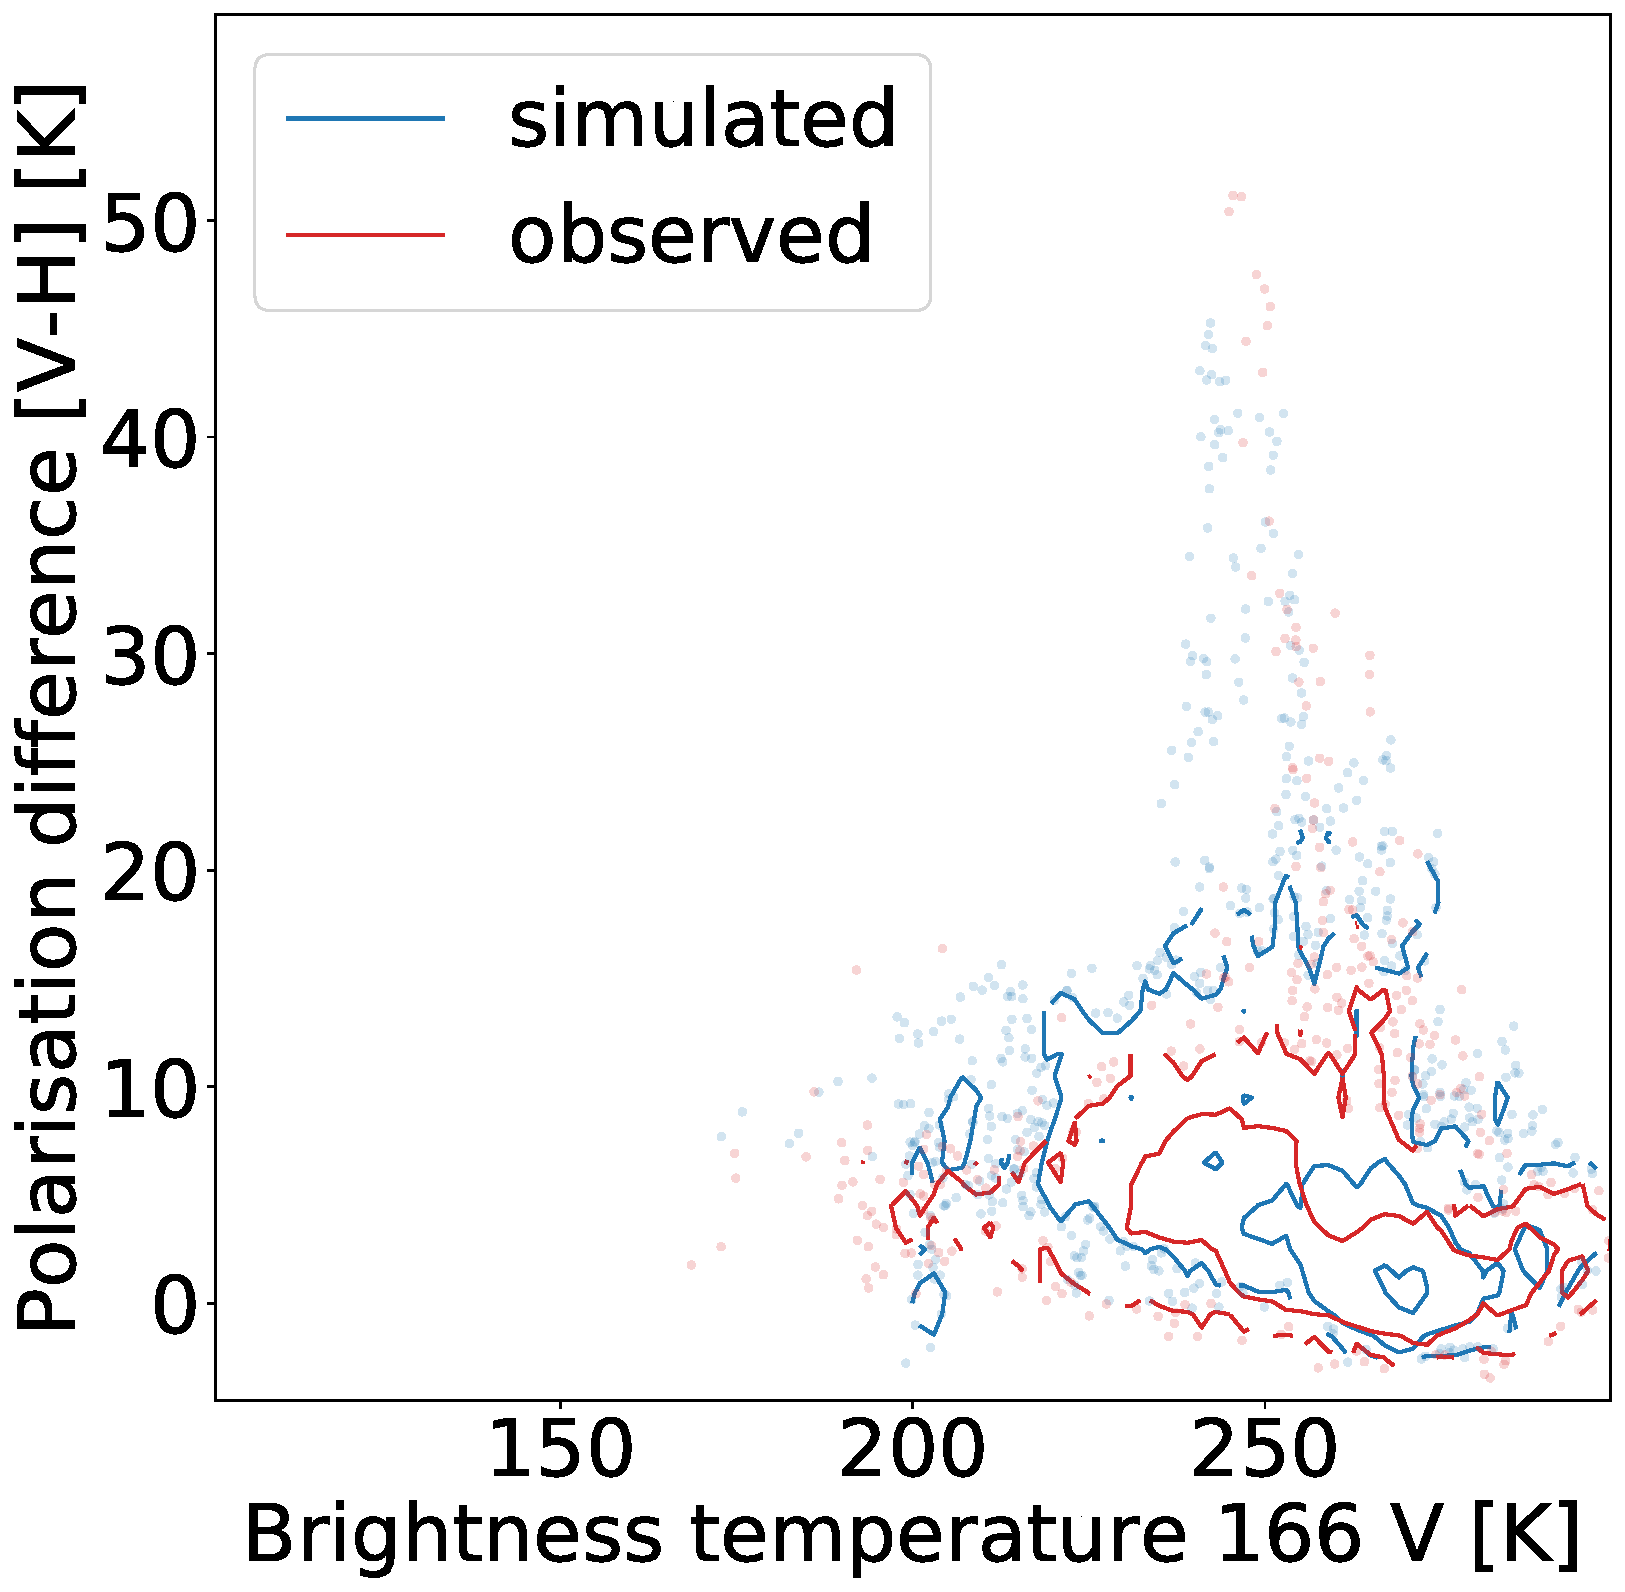
\includegraphics[height=39mm, width = 39mm]{Figures/hist2d_gmi_45-65_land.pdf}
	\end{subfigure}
	\begin{subfigure}{.24\textwidth}
		\caption{Water}
		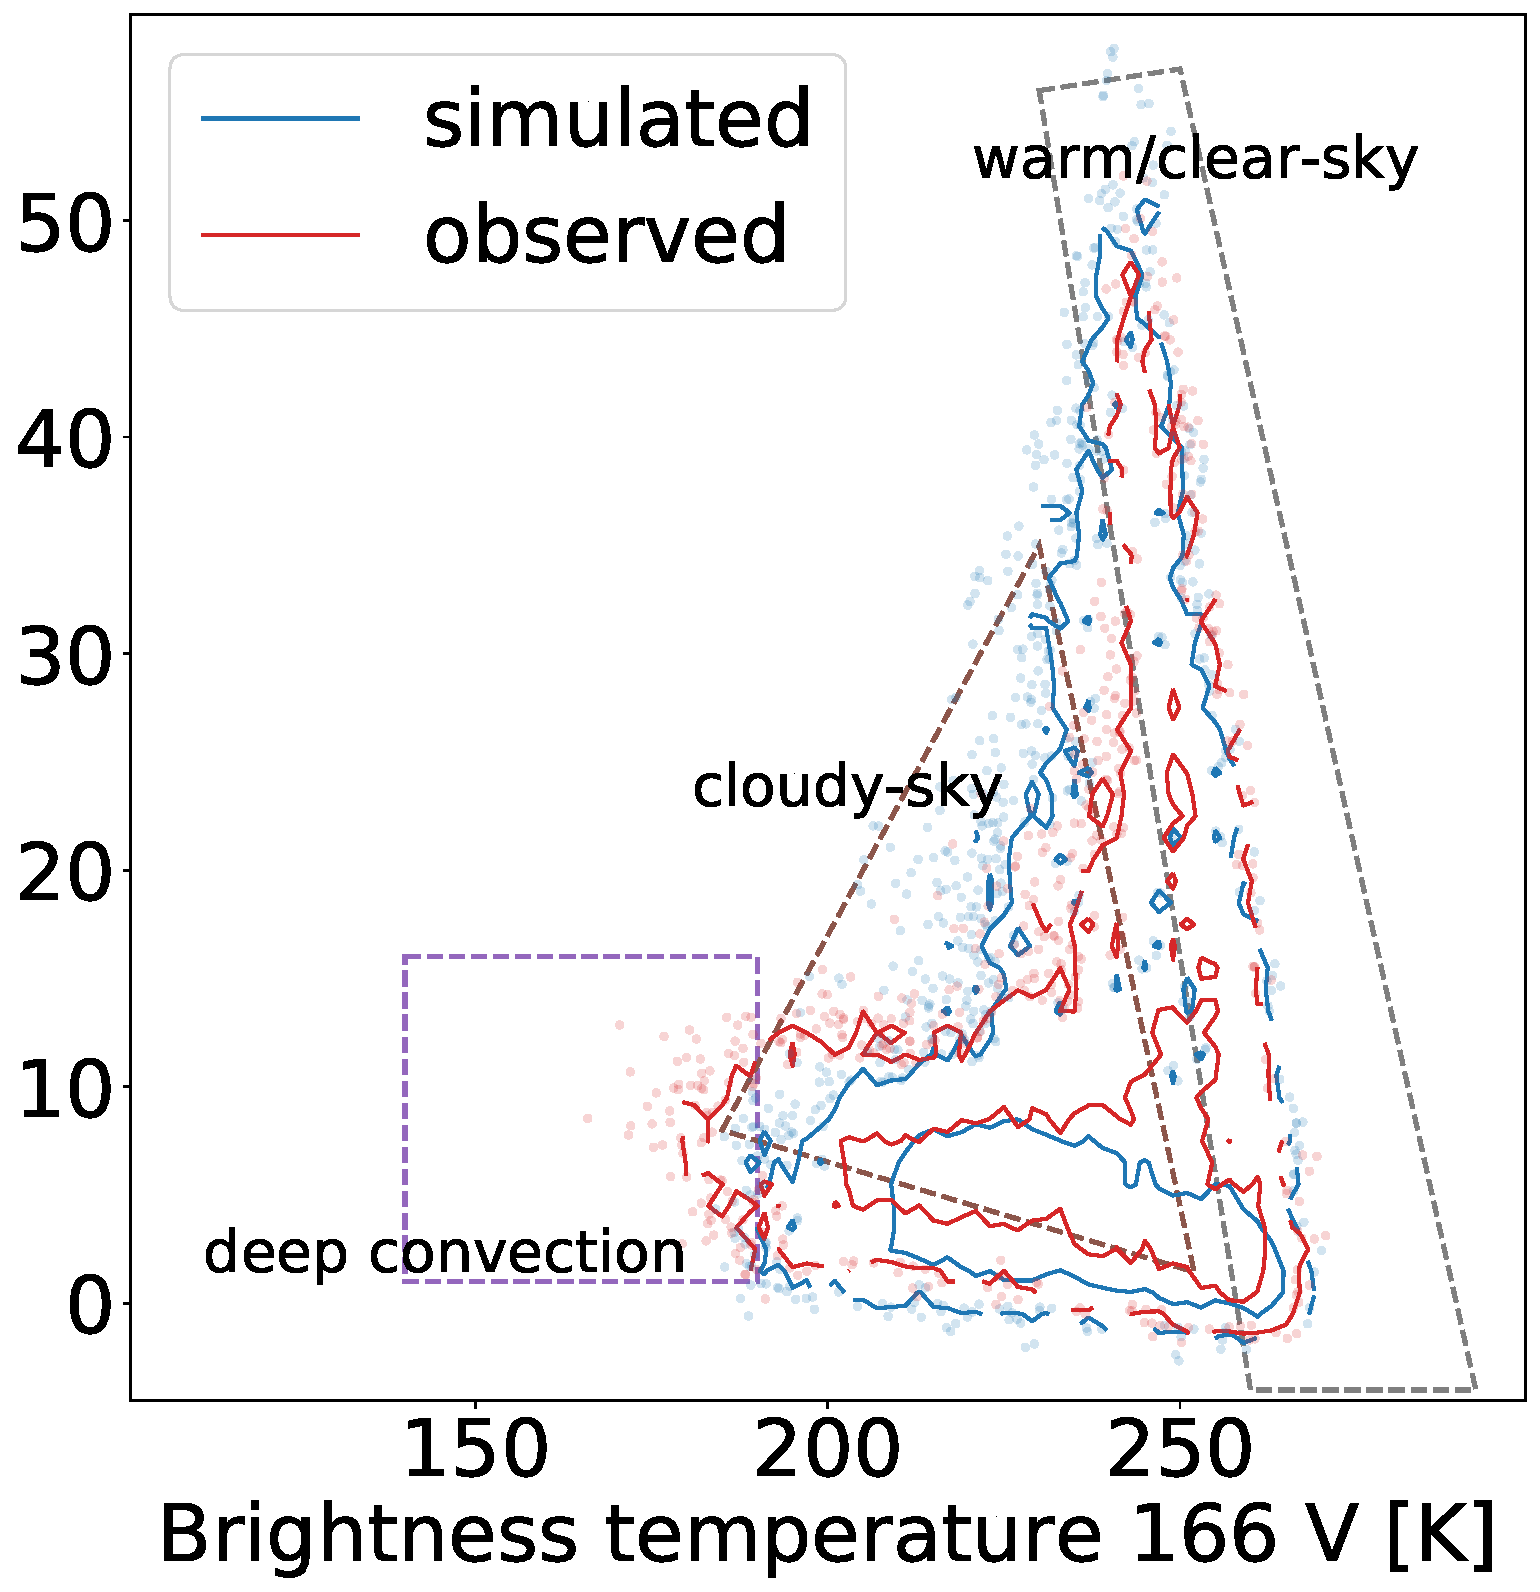
\includegraphics[height = 39mm, width = 39mm]{Figures/hist2d_gmi_45-60_sea.pdf}
	\end{subfigure}
	\begin{subfigure}{.24\textwidth}
	\caption{Snow}
	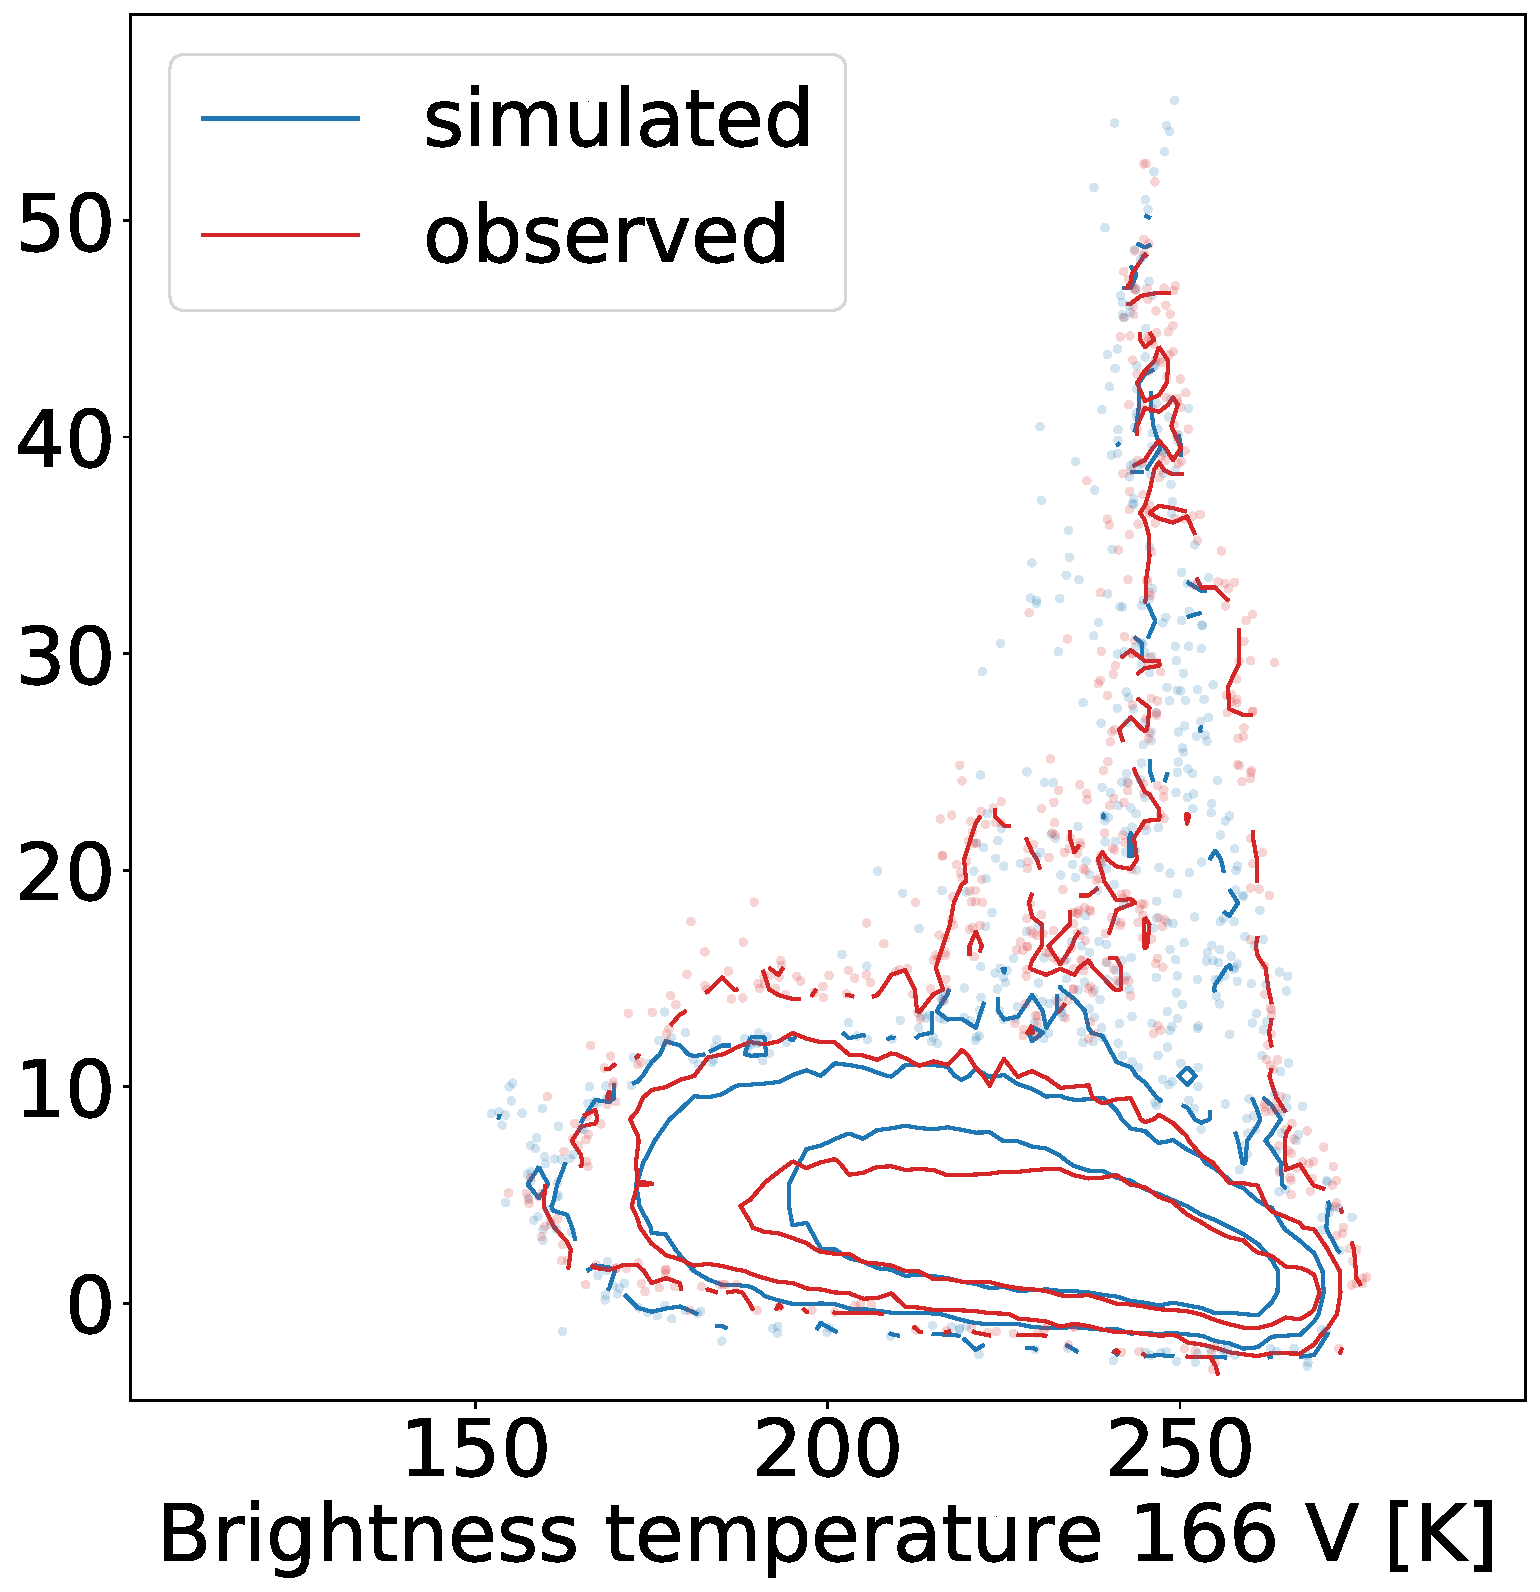
\includegraphics[height = 39mm, width = 39mm]{Figures/hist2d_gmi_45-60_snow.pdf}
\end{subfigure}
\begin{subfigure}{.24\textwidth}
	\caption{ Sea-ice}
	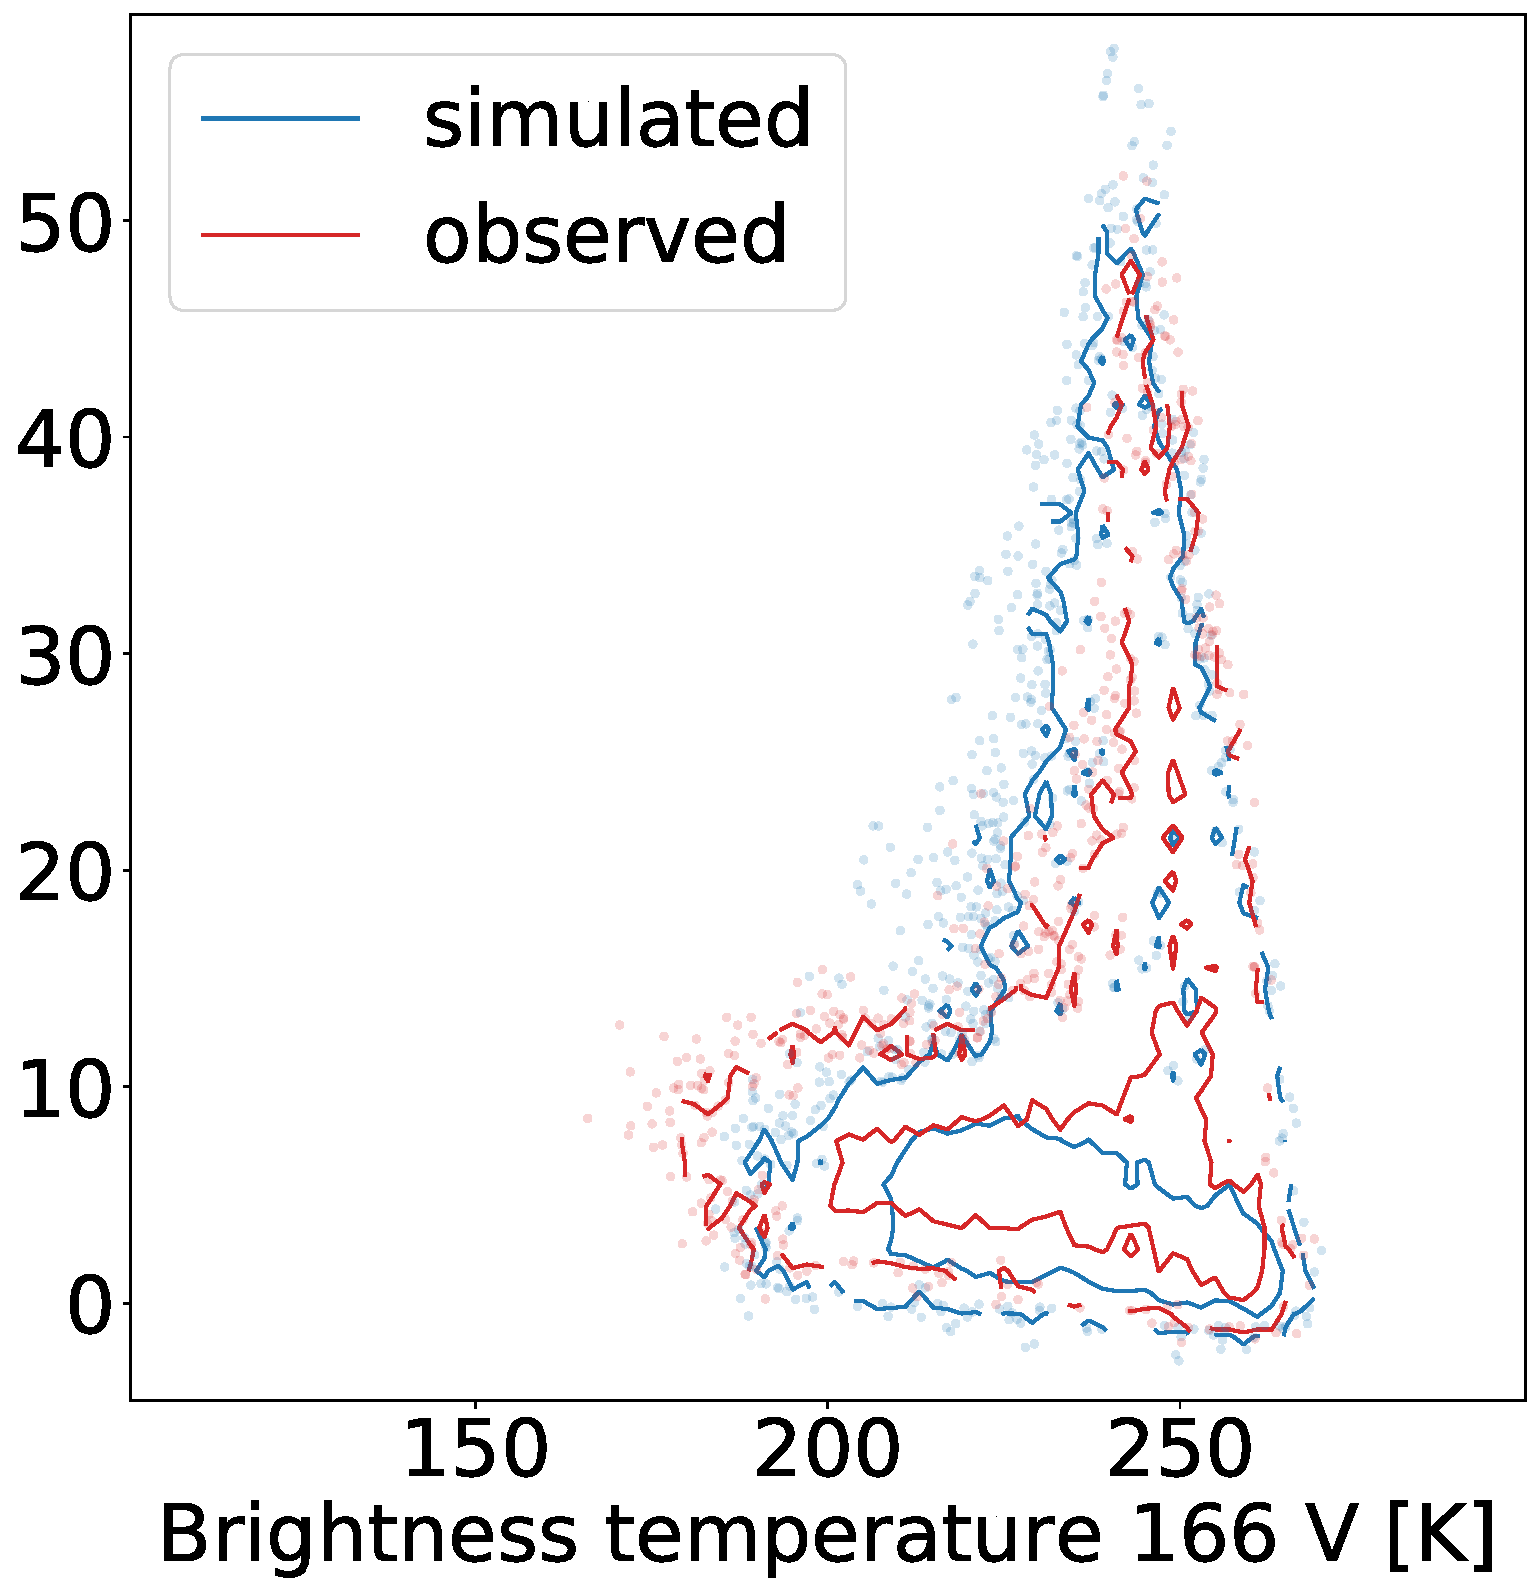
\includegraphics[height = 39mm, width = 39mm]{Figures/hist2d_gmi_highlat_sea-ice.pdf}
\end{subfigure}
\caption{Two-dimensional occurrence frequencies of 166\,GHz GMI data. The x-axis
  is the brightness temperature of the channel having vertical polarisation.
  The y-axis is the difference to the channel having horizontal polarisation.
  Figures (a)-(d) are for land, water, snow and sea-ice surface types,
  respectively. The data are from the 45$^\circ$ - 65$^\circ$ latitude bands in
  both hemispheres. In panel c, the parts of the distribution most closely
  connected to impact of the surface and hydrometeors are marked.}
  \label{fig:histogram_2d}
\end{figure*}

The training database must represent the actual measurement space, otherwise,
the retrievals associated with poorly represented cases would be inaccurate.
Accordingly, before starting with the retrievals, it is crucial to verify the
distribution of simulated measurements in the training database.
Figure~\ref{fig:histogram_2d} shows radiance histograms for the two 166\,GHz
channels, for both simulated and measured data. For all the surface types
shown, the histogram contours for both datasets overlap to a large extent. This
indicates that we simulate the polarisation signatures of all surface types and
ice hydrometeors well. There is a similar good match with observations for the
183\,GHz channels (not shown). This is an important result as we cannot expect
the retrieval to work properly unless the training database mimics the real
observation quite closely. The is true for all retrievals, not only ML. The
assumptions in traditional retrievals can be scrutinised in the same way, but
this is rarely done.

\subsubsection{Retrievals}
\label{sec:preliminary_results}
\begin{figure*}[t]
	\centering
	\begin{subfigure}{.54\textwidth}
		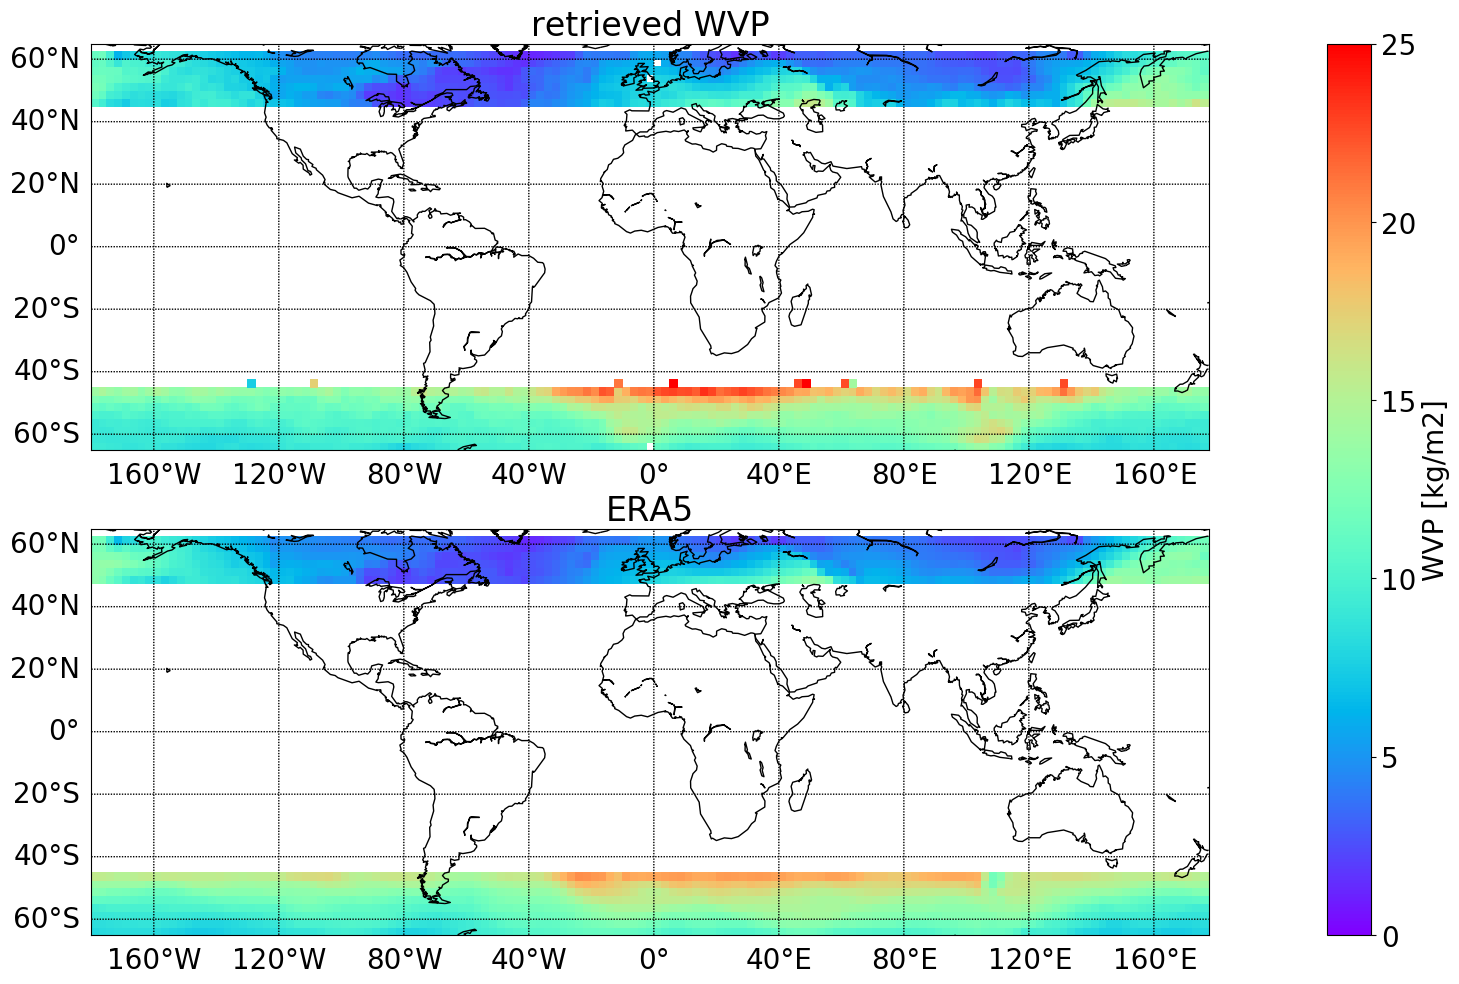
\includegraphics[height = 55mm]{Figures/WVP_spatial_jan2020.png}
	\end{subfigure}
	\begin{subfigure}{.34\textwidth}
	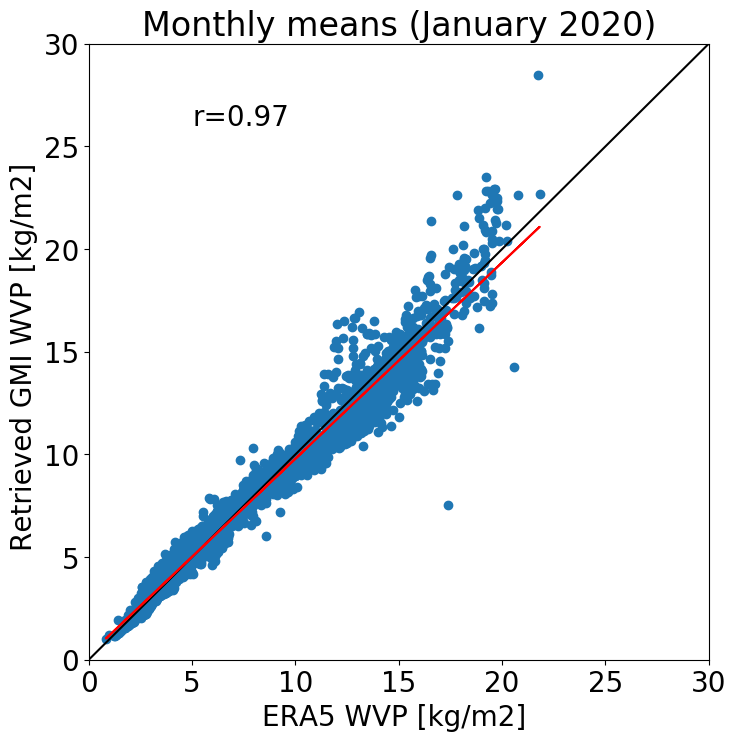
\includegraphics[height = 50mm]{Figures/WVP_scatter_monthlymean.png} 
	\end{subfigure}
	\caption{The spatial distributions (left) of monthly means estimated from retrieved WVP and ERA5 WVP. The data is for January 2020. The corresponding scatter between the two datasets is shown on the right. The red line is the line of best fit, while the black indicates the perfect fit.}
	\label{fig:WVP_retrievals}
\end{figure*}

The QRNN algorithm (Sec.~\ref{sec:qrnn}) is trained with radiances from
simulated GMI data ($\sim$500\,000 simulations) for the frequencies: 166V,
166H, 183$\pm$3 and 183$\pm$7\,GHz, to retrieve the corresponding WVPs.
Two-metre temperature, latitude and surface type are also provided as auxiliary
information. The trained net is then used to retrieve the WVP using actual GMI
measurements. A comparison of monthly means of the retrieved WVP (re-gridded at
2.5$^{\circ}$ resolution) and ERA5 reanalyses is shown in
Fig.~\ref{fig:WVP_retrievals}. The spatial distributions of both datasets
largely agree with each other, except around 45$^{\circ}$S. The presence of
these erroneous cases is not surprising; they likely occur due to the
saturation of high frequency channels in regions with high humidity. This
saturation effect will be lower when further channels are included. In spite of
the outliers, the correlation between the two datasets is 0.97.


\subsection{Work Flow}
\label{sec:wp}


The work flow is described as work packages (WPs) and the overview is displayed
in Fig.~\ref{fig:flowchart}. No Gantt chart is included as it would not be
informative. The WPs will overlap and extend over a large fraction of the
project period. The approach will be to have a first version of the retrieval
ready early (at least during year 1), analyse the results, identify the
shortcomings, and repeat the WPs accordingly. A likely situation is that the
retrievals will work less well for one surface type, or that including some
channels deteriorates the accuracy, necessitating the reiteration of one or
several WPs. The project will require extensive calculations, but the
computational resources available from Chalmers central cluster (C3SE) and
locally inside the division will meet the demands with margin

\begin{figure}
	\begin{minipage}[c]{0.75\textwidth}
		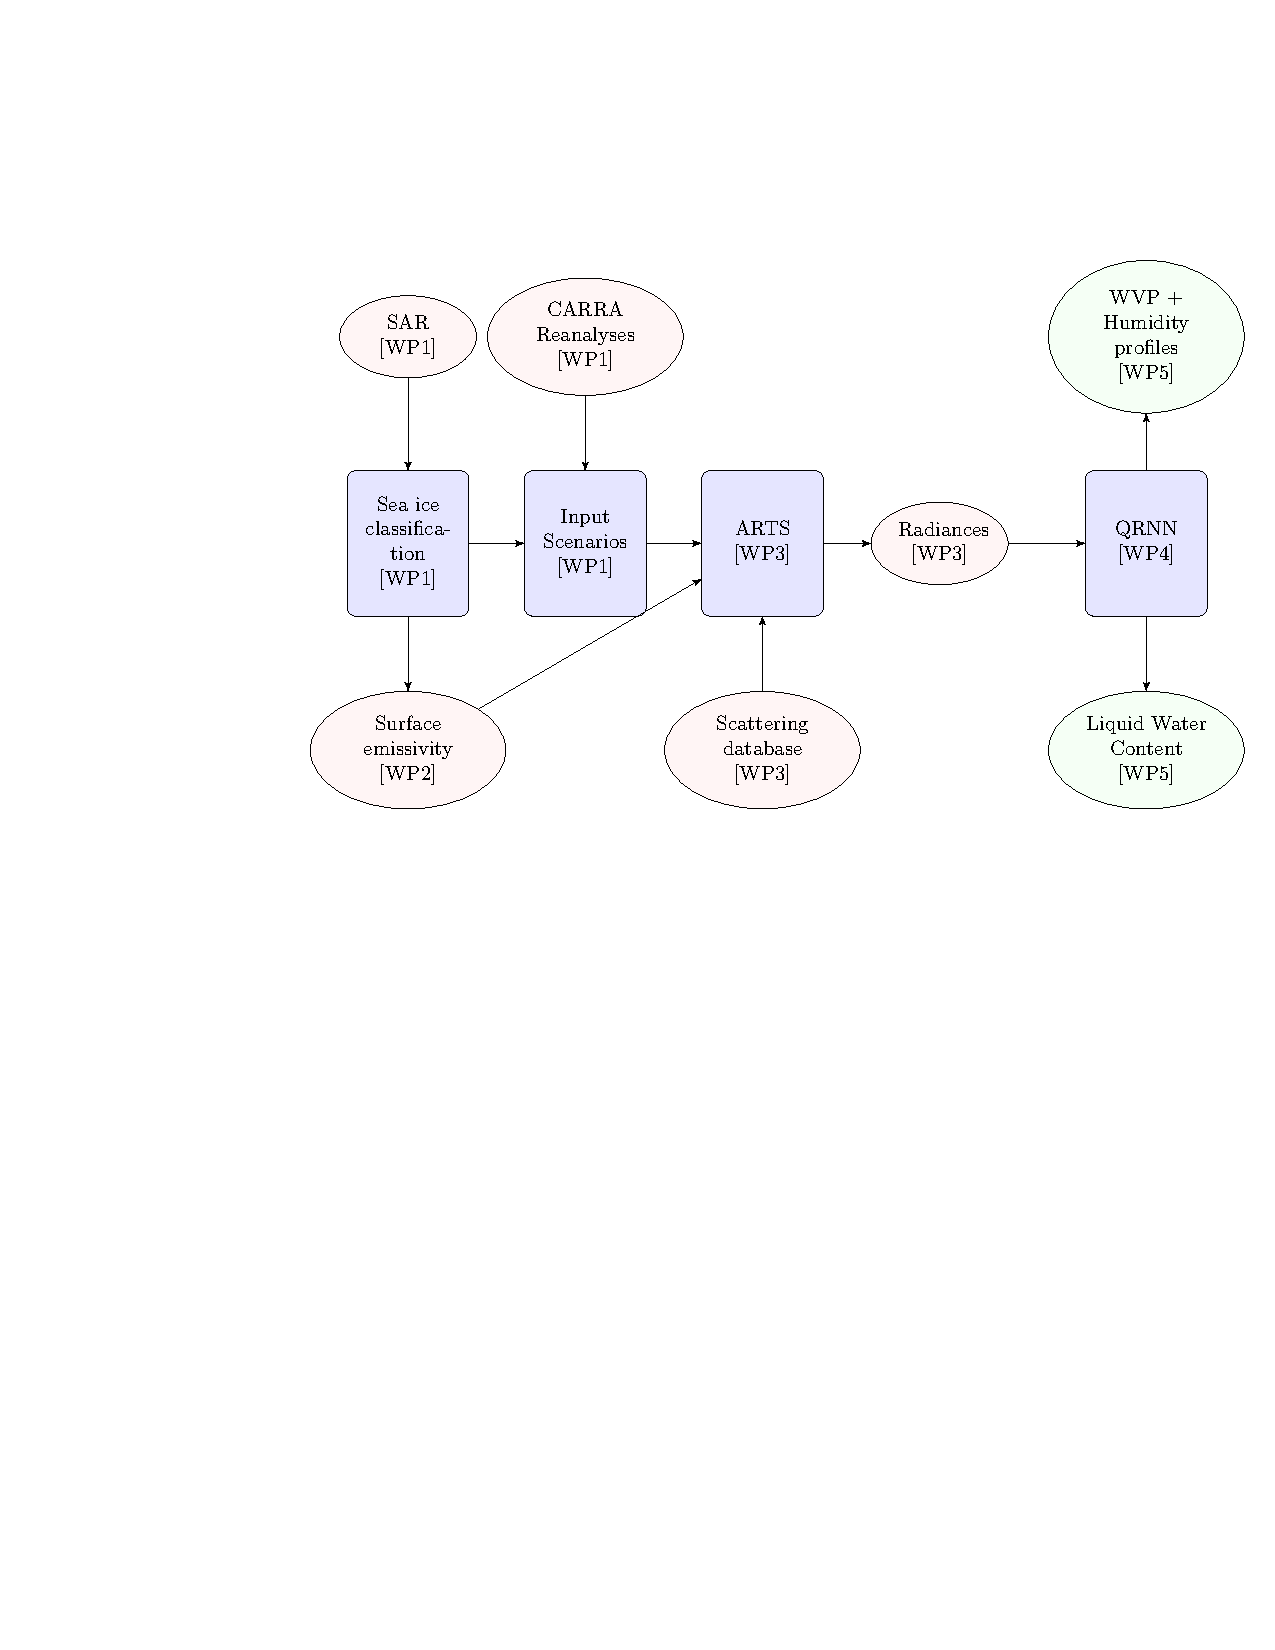
\includegraphics[trim=100 400 15 125,clip,height = 50mm, width=100mm]{flowchart.pdf}
	\end{minipage}\hfill
	\begin{minipage}[c]{0.24\textwidth}
      \caption{Flowchart of the proposed retrieval system. The green boxes
        represent the retrievals. Only WPs 1-5 are shown. WPs related to
        evaluation (WP~6) and additional retrievals (WP~7) are not shown.
      } \label{fig:flowchart}
	\end{minipage}
\end{figure}

\vspace{-1ex}
\subsubsection*{WP 1: Basic atmospheric scenarios}
%

\label{sec:atmscenes}
The inputs to the forward model can be based on either atmospheric models
providing a sufficiently detailed description of hydrometeors, or on
measurements \citep{ekelund:using:20}. In this study, we will adopt the former
approach and use reanalyses from CARRA (see Sect.~\ref{sec:harmonie}) to create
a database of the atmospheric cases. CARRA does not cover all the Arctic
regions, so if needed, reanalyses from ERA5 will be included. Furthermore, use
of high-resolution SAR imagery to characterize the sea-ice/open waters will be
made (see Sect.~\ref{sec:sar}). The fine spatial resolution of SAR will
facilitate better mapping of inhomogeneous surface types, and thus reduce
errors with respect to mixed surface types such as polynyas. To our best
knowledge, this shall be the first instance where such high-resolution
information would be used in this context. The output of this work package will
be a broad set of 3D scenarios, based on collocated SAR and CARRA data, to be
used as input to the radiative transfer simulations. \vspace{-1.0ex}

\subsubsection*{WP 2 : Emissivity model}
%
\label{sec:emissivity}
An important step is the estimation of the surface emissivity spectra over a
multitude of surface types. As a first step, we will consider using existing
studies to extend the snow-emissivity model (see Eqs.~\ref{eq:1}- \ref{eq:2})
to lower frequencies such as 89\,GHz and 50\,GHz. Such an empirical model will
be easy to fine-tune by comparing observed and forward modelled radiances. Also
optimal estimation retrievals (with ARTS) will be explored. A joint retrieval
of the emissivity spectrum over all frequencies will be made. The basic idea is
to find a set of emissivity estimates for all the considered frequencies that
would simultaneously give radiance closest to the measurements. Such retrievals
should be especially useful to understand the correlation of emissivity
variations between frequencies; thus making it more viable from an assimilation
perspective. The retrievals in this WP will be made assuming both specular and
lambertian reflection. The differences between the two more or less vanish for
conical scanners, while for cross-track scanners, a combination of the two is
used to characterize realistic surfaces \citep{matzler:2005:onthe}. The
observed and simulated radiances will be compared to judge exactly what
combination works best for various surface types and incidence angles.

The output of this work package will be an empirical, statistical model of
snow emissivities. If found needed there will be two models, one for snow on
land and one for snow/sea-ice. This WP could potentially result in a separate
journal article.
\vspace{-1.0ex}

\subsubsection*{WP 3 : Database creation and post-processing}
%
\label{sec:database}	
This WP covers the initiation and execution of the batch radiative
transfer calculations. Initially, some time will be spent on to implement the
scripts needed for the basic calculations, to add jobs to the calculation
cluster, and post-processing. As a start, only conical scanners will be
simulated, and later extension to cross-track scanners will be made. For the
latter, a number of scan angles, between nadir and swath edge, will be covered.

ARTS will be applied to generate simulated observations, based on the data and
models from WP 1 and WP 2. For both types of scanners, overlapping antenna
footprints of all frequencies will be explicitly simulated. To generate the
antenna pattern at the desired frequency, a number of pencil beam radiative
transfer calculations will be performed to incorporate both along-track and
across-track sampling. To also account for imperfect calibration of the
instruments, bias adjustments as calculated by ECMWF will be considered as a
post processing step. Sensor calibration and its relative agreement with the
forward model are vital for the success of the retrieval database. The WP
output will be batches of simulated radiances.  \vspace{-1.0ex}


\subsubsection*{WP 4 : Retrieval setup}
%
\label{sec:setup}
The retrievals will be made without introducing any re-mapping of the satellite
measurements. All footprints inside a region would be used as input, following
the size of the simulated scenes in the database generated in WP 3. This
approach will make much better use of the spatial information provided by the
overlap of instrument footprints. The target resolution will not be
compromised and retrievals can be made at the highest possible resolution,
while preserving the information at their native resolution. This has been
demonstrated using 2DVAR in \citet{duncan:anexp:19}. But here we shall aim to
achieve the same purpose by using QRNN. In fact, using QRNN is even more advantageous as it does not require any explicit calculation of the spatial correlations through covariance matrices as in 2DVAR.
%a retrieval database
%(and not 2DVAR) does not restricted to describe spatial correlations by
%covariance matrices and the QRNN version should be even more advantageous.

QRNN is already available as a part of the Typhon software package
\citep{lemke:2020:typhon}. The implementation of the retrieval algorithm shall
be straightforward but it will be important to find the
neural-network architecture and auxiliary data required to achieve the best model performance.



\vspace{-1.0ex}
\subsubsection*{WP 5 : Retrievals}
%
\label{sec:retrievals}
%
In this WP, firstly we will extend our preliminary results for WVP (see
Sect.~\ref{sec:preliminary_results}) to include regions north of 65$^\circ$,
using SSMIS. An extension to lower frequencies, such as 89\,GHz and channels
around 50\,GHz, will be tested. Including the latter can be beneficial to
resolve the low-level cloudiness. In fact, the estimates of liquid water
content/path and WVP are not completely independent. The synergies between the
two quantities will be exploited to correct the estimates for each other.
Inclusion of 22\,GHz and 37\,GHz to increase sensitivity to high humidity
regions could also be considered, though on a lower priority. These channels
are more important over open-waters than sea-ice regions. The ultimate goal
will be to include sufficient channels such that the full information content
of tropospheric water is preserved. In the second step, the scheme will be
extended to ATMS, a cross-track scanner. Here a larger database covering the
various incidence angles will be used, but we will focus on the central part of
the swath and avoid the large footprinst further out in the swath. With ATMS
five 183\,GHz channels are at hand. This gives a better constrain of the
vertical domain and also humidity profiles will be retrieved (by QRNN):
%For LWC over sea-ice, the combination 89+150\,GHz would be tried as has been suggested by \citet{laue:2007:poten}.
%Later, the best channel combinations will also be used to estimate the
%humidity profiles. 
%The pivotal part of these retrievals would be using ML on the overlapping footprints to extract the hidden information without any explicit treatment.

This WP will run concurrently with WP 3 and WP 6. We will set-up test retrievals as soon as few hundred thousand simulations are available, so that an early feedback on any database issues can be made. Besides, during the development phase, a basic evaluation (see Sect.~\ref{sec:evaluation}) of the retrievals with existing retrieval products will be made to identify the areas requiring improvement. Repetition of the retrievals will be made accordingly.

The output of this WP will be one or more retrieval databases for WVP, humidity
profiles and liquid water path.
\vspace{-1.0ex}

\subsubsection*{WP 6: Evaluation and dissemination}
%
\label{sec:evaluation}
The primary task of this WP will be to evaluate the quality of the retrievals.
This would be done by comparisons with other existing products,
satellite-based, in situ and reanalyses. Statistical comparisons will be made,
e.g,\, time series analysis of daily and monthly means, and comparisons of the
probability distribution functions. Comparisons over seasons and different
surface types will also included. In the first stage, this WP would focus on
identifying and understanding the areas of shortcomings so that the next
iterations of the retrievals can be improved. This WP will also serve as an
indirect evaluation of the emissivity model in WP 2. Within a two-year time
frame, we will likely not have time to apply the data ourselves for e.g.\
climate model evaluation, but efforts will be made to promote such applications.
%A thorough investigation with the available \textit{in-situ} data,
%satellite products and reanalysis will be made. Firstly, direct comparisons
%with radio-soundings or data from flight campaigns will be used to estimate the
%accuracy of the product and reveal the uncertainties on finer scales.
%Statistical comparisons with other microwave and IR based humidity products
%will also be made. Time series of daily and monthly means, and the probability
%distribution functions of the retrievals will be analysed. Here it would also
%be important to analyse the accuracy over seasons and different surface
%types.The evaluation part shall also go hand-in-hand with the retrieval WP.
The dissemination of the retrieved dataset will also be through conferences and
journal articles. The assessment of how well the produced dataset answers the
needs of NWP communities will also be addressed through collaborations with
ECMWF and the Swedish Meteorological and Hydrological Institute (SMHI). See
also Sec.~\ref{sec:collaborations}.
\vspace{-1.0ex}
\subsubsection*{WP 7 : Additional Retrievals}
%
\label{sec:other_retrievals}

If the work around humidity and liquid water content progresses fast, we will
also consider retrieving snowfall and sea-ice concentration. The extension of
QRNN to these parameters will be straightforward, requiring only a change in
training target, but some work will be required to optimize the training and
find the best combination of auxiliary data. Among the two, snowfall retrievals
will be considered first.
%
 
\subsection{Risk Assessment}
%
\label{sec:risk}
All activities planned in this project are a direct continuation of ongoing
work and the level of risk in the basic work plan can be judged as low. The
calculation of emissivity spectra over sea-ice and heterogeneous regions is
often considered difficult and neglected. However, with use high resolution SAR
data and a pragmatic, statistically-based, approach for modelling emissivities,
there are no ``showstoppers''. We can gradually improve the emissivity model,
based on the observational data alone. 

Usage of low frequencies like, 22 and 37\,GHz should be seen as more
speculative considering their large footprint size, but their inclusion has low
priority. As mentioned, the existing access to computational resources meets
the demands raised by the project.


\section{Impact and social benefits}
%
\label{sec:impact}

As a society, understanding the weather and climate processes in the polar
regions are important to tackle the effects of climate change, and also to
improve mid-latitude weather forecasts. The anthropogenic climate change over
poles also has economic and political implications, e.g. commercial
navigational activity through the Arctic, which requires accurate weather
forecasts to avoid accidents and oil spills.

The overall retrieval procedure requires a deep understanding of the physics
governing the observed radiances. This knowledge can be shared with the NWP community and an indirect significant impact of the data on weather forecasting can be expected. Work towards amplifying the ingestion observations in NWP will be covered in association with modelling community at SMHI and ECMWF (Sec.~\ref{sec:collaborations}).


%A consistent database of standalone retrievals
%is important for NWP, which rely on satellite based retrievals to determine the
%initial atmospheric conditions. Additionally, the sea-ice emissivity estimates
%can be used to reduce the forward model errors arising due to surface
%contribution in radiative transfer.


\section{Collaborations}
%
\label{sec:collaborations}
The retrievals will be made publicly available and we will actively search
for cooperation inside the climate modelling community to ensure that the 
data will be applied for verification of models and similar activities. For example, we will reach out to the group of Prof. Johannes Quaas at Leipzig University. 

%Johannes Quaas group at Leipzig university, ICON; Corinna Hooses group at KIT, Karlsruhe, ICON-ART;  there are also people in Bremen and at AWI working at the sea-ice atmosphere interaction/water vapour,

The experience obtained in the project can be transferred to the NWP community
by existing contacts. Patrick Eriksson has an established collaboration with
SMHI (around ICI and QRNN), and AWS should broaden the contact. For example,
discussions are ongoing on how Chalmers can contribute to the upcoming
``Nordic AWS study''. Further, Patrick and Leif Eriksson are co-applicants in a
proposal from SMHI, also submitted to SNSA 2021-R. The title of that proposal
is ``Consistent Air-Ice-Sea Data Assimilation of Satellite Observations`` and
there are high similarities between the projects.

The EUMETSAT fellowship hold by V.\ Barlakas has established a direct
collaboration with ECMWF \citep{barlakas:intro:21}. Furthermore, the interest
in the research performed at Chalmers has resulted in an appointment of Patrick
Eriksson as an ECMWF fellow\footnote{See 
	\url{www.ecmwf.int/en/about/media-centre/news/2020/ecmwf-appoints-seven-new-fellows-scientific-collaboration}}.
Another contact at ECMWF is through David Duncan (former post doc at Chalmers).
He contributed to the recent study by Inderpreet Kaur, and this contact will be
maintained.



\section{Staff situation}
%
\label{sec:staff}
Inderpreet Kaur started as a postdoctoral researcher in the division in March
2020. She is presently working with retrieval of atmospheric ice hydrometeors
using microwave instruments. She shall spend 80\,\% of her time towards the
project. Patrick Eriksson will contribute to all WPs and act as overall project
leader. Luisa Ickes is an Assistant Professor, and has the Arctic region as her
special research interest. She will provide expertise in cloud physics and the
conditions in the Arctic region in general, both when generating training data
and evaluating retrievals (WPs 1, 5 and 6). Leif Eriksson is an Associate
Professor and his research aims at developing methods to observe land and ocean
properties with radar data. In this project, his expertise is sought on the use
of SAR data. He will mainly contribute to WP 1. The
last three persons will spend at least 5\,\% of their time on the project.
During 2022 this will level be 10\,\% for Leif Eriksson. See further Cost
Specification enclosure.


\section{Satellite data}
%
All satellite data of concern in this project are publicly available. SSMIS
data can be obtained at
\url{www.ncei.noaa.gov/access/metadata/landing-page/bin/iso?id=gov.noaa.ncdc:C00810},
and\\ATMS data are available at \url{ftp-npp.bou.class.noaa.gov/}. SAR data from Sentinel-1 are freely  available from the Copernicus Open Access Hub https://scihub.copernicus.eu

{\footnotesize
	\bibliography{j_abbr,refs_pe1,references}
}
\end{document}
